%%%%%%%%%%%%%%%%%%%%%%%%%%%%%%%%%%%%%%%%%%%%%%%%%%%%%%%%%%%%%%%%%%%%%%%%%%%%
\documentclass[a4j,11pt]{jarticle}           % pLaTeX の場合
\usepackage{authblk}
\usepackage[dvipdfmx]{graphicx} 

% usepackage置場 TODO
\usepackage{cite}
%\usepackage[dvips]{graphicx}
\usepackage{amsmath}
\usepackage{amssymb}
\usepackage{marvosym}
\usepackage{pifont}
\usepackage{ascmac}
\usepackage{url}
\usepackage{booktabs}
\usepackage{float}
\usepackage{comment}
\newcommand{\argmin}{\mathop{\rm arg~min}\limits}
% \setlength{\oddsidemargin}{1.0cm}
% \setlength{\evensidemargin}{1.0cm}
\renewcommand{\floatpagefraction}{0.7}
\renewcommand{\baselinestretch}{1.3}
\renewcommand{\arraystretch}{0.8}
\renewcommand{\refname}{文献}
% \newcommand{\Nnm}{${\rm N_{n,m}}$}
\pagestyle{empty}
\bibliographystyle{prml}
%%%%%%%%%%%%%%%%%%%%%%%%%%%%%%%%%%%%%%%%%%%%%%%%%%%%%%%%%%%%%%%%%%%%%%%%%%%
\begin{document}
	\begin{titlepage}
		\setcounter{page}{0}
		\begin{center}
			\vspace*{2.0cm}
			\LARGE
			%タイトル
			ユーザーの好みに合ったモデルを用いた\\レコメンデーション\\
			\vfill
			%title(English)
			Factor-Controlled Recommendation for \\Visualizing User's Preference
			\vfill
			\LARGE
			北海道大学 工学部\\
			情報エレクトロニクス学科\\
			情報理工学コース\\
			情報認識学研究室
			
			\vspace{2ex}
			%名前
			茅根 宏介\\
			\vspace{2ex}
			%日付
			2020年3月\\
			\vspace*{2cm}
		\end{center}
	\end{titlepage}
	\tableofcontents \thispagestyle{empty}
	\newpage
	\listoffigures
	
	\listoftables
	\clearpage 
	\pagestyle{plain} 
	
	%%%%%%%%%%%%%%%%%%%%%%%%%%%%%%%%%%%%%%%%%%%%%%%%%%%%%%%%%%%%
	%platexでコンパイル
	%%%%%%%%%%%%%%%%%%%%%%%%%%%%%%%%%%%%%%%%%%%%%%%%%%%%%%%%%%%%
	
	\section{はじめに}
	\subsection{研究背景}
	推薦システムは, 近年多くのwebサービスにおいて使われていて, ユーザーにとって有用と思われるアイテムを選び出し,  それをユーザーの目的に合った形で提示する\cite{rec1}\cite{rec2}\cite{rec3}. 協調フィルタリング\cite{cf}などの従来の多くの方式がユーザーの購買履歴などのユーザーとアイテム間の情報のみを扱っている. 最近では, webサービスが急速に発展し, Spotify\footnote{https://www.spotify.com/jp/}やNetflix\footnote{https://www.netflix.com/jp/}などのソーシャルメディアが普及し, 
	利用できる情報が増えた. 例えばソーシャルメディアでは, ユーザー同士が友達関係を作ったり, ユーザーがアイテムにタグを付けることができる. これらのソーシャル情報は推薦システムにおいても有益であることが知られている\cite{social}\cite{tag}.しかし, それらの複雑な情報をモデル化し推薦に用いることは困難とされてきた.
	そこで, ソーシャル情報を柔軟に扱う手法としてHeterogeneous Information Network (HIN)\cite{HIN}やハイパーグラフ\cite{hyper}を用いることで様々なオブジェクトや関係性を扱う手法が開発された. 
	\\ HIN\cite{HIN}やハイパーグラフ\cite{hyper}を用いた手法ではユーザーとアイテム間などの関係性をエッジを用いて表現する. ソーシャルメディア上には関係性が何種類か存在するので, 
	エッジの種類も複数存在し, 各々が重要な意味を持つ. そこで, それぞれの種類のエッジに重みを付けることで, 関係性の重要度とユーザーの好みを表現することを考える. 
	しかし, HIN\cite{HIN}を用いたHete-CF\cite{Hete}やハイパーグラフ\cite{hyper}を用いたMusic Recommendation via Hypergraph(MRH)\cite{MRH}では, 
	エッジの重みでユーザーの好みを表現できない. 
	
	\subsection{本論文の目的}
	本論文では, ソーシャル情報であるユーザーやアイテム, タグなどの複数のオブジェクトとそれらの関係性を用いることで, ユーザーの好みを表現するパーソナライズな推薦を提案する. 
	具体的には, ソーシャル情報をハイパーグラフを用いてモデル化し, 関係性を表現するエッジの重みを調整することで, 推薦結果における推薦因子の寄与分を変化させ, 
	推薦モデルがユーザーの好みを反映した推薦を実現する. エッジの重みが異なる推薦モデル間において, 推薦因子の寄与分と個々のユーザーの推薦の精度の変化について実験により調査する. 
	ユーザーによって最適な推薦因子の寄与分が異なることを検証し, 推薦モデルがユーザーの好みを表現するパーソナライズな推薦を可能にする. 
	
	\subsection{本論文の構成}
	本論文は本章を含め7章で構成する. 第2章ではソーシャル情報を柔軟にモデル化し, 異なるオブジェクト間の関係性をエッジで表す手法についての従来研究を挙げる. 第3章では, 提案手法がベースとした推薦手法MRHを紹介する. 第4章ではユーザーの好みを表現するパーソナライズな推薦を提案する. 第5章では, 実験の結果を示し, 第6章ではその考察を行う. 最後に第7章では, 本論文の結論と今後の方針について述べる. 
	\newpage
	\section{従来研究}
	ソーシャルメディア上には, ユーザーやアイテム, タグなどの複数のオブジェクトとそれらの関係性などの複雑な情報が多く存在する. 
	そこで, これまで行われてきたそれらの関係をモデル化する手法を紹介する. 
	\subsection{Heterogeneous Information Network}
	Heterogeneous Information Network (HIN)\cite{HIN}は, オブジェクト間の関係性をグラフによって表現する手法である. 
	例えば, ノードとして表現するユーザーとアイテム間における購買履歴などの関係性をエッジにより表現する. ソーシャルメディア上には関係性が何種類か存在するので異なる種類のエッジも複数考える. HIN\cite{HIN}は類似検索やクラスタリング, 分類問題などの分野において用いられている. 
	\\ Hete-CF\cite{Hete}は,HIN\cite{HIN}を用いた推薦方式であり, ユーザー間の関係, アイテム間の関係に加えて, ユーザーとアイテム間の3つの関係を用いて推薦している. 
	推薦モデルを最適化する際, それぞれの関係に重みに関するパラメータが存在する. 推薦の精度について, ユーザーとアイテム間の関係である評価情報をどのくらい考慮するかというパラメータに依存する. レーティング情報が少ない時, そのパラメータを大きくすることで精度が上がり, レーティング情報が多い時には偏りが生じてしまうのでパラメーターを小さくすることで精度が上がる. 
	このように, 精度はユーザーとアイテム間の関係をどのくらい考慮するかという点に依存する. 
	\subsection{ハイパーグラフ}
	ハイパーグラフもHINと同様にオブジェクトの関係をグラフで表現したものであり, 3項以上の関係を表すハイパーエッジを用いるため, 対の関係よりも複雑な高次関係をモデル化できる. 従来よりクラスタリングや分類問題などの分野で利用されてきた\cite{hyper}. Music Recommendation via Hypergraph (MRH)\cite{MRH}はこのハイパーグラフを推薦に利用している. 詳しくは第3章で述べるがMRH\cite{MRH}は, ソーシャル情報をハイパーグラフを用いてモデル化し, ランキング問題の最適化を解く際, 
	ハイパーグラフの辺の重みを考えて推薦を行う手法である. 各々のユーザーに対しランキングスコアが高いアイテムほど, そのユーザーとの関連度が高くユーザーの好みに合った推薦が行われる. MRH\cite{MRH}も, 異なるオブジェクト間の関係性をエッジを用いて表現しているが, すべてのエッジの重みが正規化され, すべての関係性が同等に考慮されている. 
	\newpage
	\section{MRH}
	本研究では, MRH\cite{MRH}をベース手法として用いる. 種々のオブジェクトとそれらの関係性をどのようにしてハイパーグラフでモデル化するか, 
	また, どのようにランキング問題を解くか説明する. 
	
	
	\subsection{ハイパーグラフ}
	ハイパーグラフを3組$G(V,E_h,w)$で表す. $V=\{v_1,v_2,...,v_{|V|}\}$はノードの集合,  $E_h$はハイパーエッジの集合である. ハイパーエッジ$e\in{E_h}$は, 通常のエッジを一般化したものであり, Vの2ノード以上の部分集合である. wは重み関数で$w:E\rightarrow (0,\infty)$と定義し, 大きい重みほど頂点間の関係が大きいことを示す. 
	また, VにはR種類, $E_h$にはS種類の区別が存在し, それぞれ$V^{(r)}(r=1,2,...,R)$, $E_h^{(s)}(s=1,2,...,S)$と表す. 映画のソーシャルメディアを例に考えると,  
	ユーザーや映画, タグなどのオブジェクトがノード$V^{(r)}$, ユーザーが映画に付ける評価情報やタグなどの関係性をハイパーエッジ$E_h^{(s)}$としてハイパーグラフが構築される. 
	\\ 次に,  ハイパーグラフに関する行列表現を定義する. まず, 接続行列$\textbf{H}\in \mathbb{R}^{|V|\times |E_h|}$はノードvとエッジeの関係を示し, $v\in{e}$ならばHの$h(v, e)$要素は1をとり, それ以外は0をとる. $|E_h|\times |E_h|$の対角行列である重み行列$\textbf{W}_h$は各々のエッジの重み$w(e)$を示す. さらに, ノードとエッジの次数$d(v)$と$\delta(e)$を成分とした対角行列をそれぞれ$\textbf{D}_v$, $\textbf{D}_e$とする. ここで, ノードvの次数$d(v)$とエッジ$e$の次数$\delta(e)$を以下のように定義する. 
	
	\begin{eqnarray}
		d(v)&=&\sum_{e\in E_h}w(e)h(v,e), \\ \delta(e)&=&\sum_{v\in V}h(v,e). 
	\end{eqnarray}
	
	
	
	
	\subsection{ランキング問題の最適化}
	推薦方式は, 複数のアイテムをまとめて推薦する場合と順位をつけて推薦する場合がある. ここでは後者, つまりランキング問題を考える. クエリベクトルを$\textbf{y}=[y_1,y_2,...,y_{|V|}]^T$としランキングスコアベクトルを
	$\textbf{f}=[f_1,f_2,...,f_{|V|}]^T$とする. ここでTは転置を表す. クエリベクトルはユーザーの好みを表す初期値ベクトルである. 
	クエリベクトルの詳細は第5.2章で述べる. また, ランキングスコア$\textbf{f}$の評価関数を以下のように定義する. 
	
	\begin{eqnarray}
		\textbf{Q}(\textbf{f})&=&\frac{1}{2}\sum_{i, j=1}^{|V|}\sum_{e\in E_h}\frac{w(e)h(v_i, e)h(v_j, e)}{\delta(e)}\left|\left|\frac{f_i}{\sqrt{d(v_i)}} - \frac{f_j}{\sqrt{d(v_j)}}\right|\right|^2 \nonumber \\ &+& \mu\sum_{i=1}^{|V|}\|f_i-y_i\|^2.
	\end{eqnarray}
	ここで, $\mu>0$は正則化パラメータである. この評価関数における最適なランキング$\textbf{f}^*$は$\textbf{Q}(\textbf{f})$を最小にする\textbf{f}である. 
	
	\begin{equation}
		\textbf{f}^* = \argmin_{\textbf{f}} \textbf{Q}(\textbf{f}). 
	\end{equation}
	
	評価関数\textbf{Q}(\textbf{f})の第1項は重みの大きいハイパーエッジを共通して多く持つ2頂点$v_i$, $v_j$のランキングスコア$f_i$, $f_j$が近いほど\textbf{Q}(\textbf{f})が小さくなる. 
	例えば, ある2つの映画i, jが多くの共通するユーザーによって好評価されていた場合にそれらの映画i, jの最適なランキングスコア$f_i$, $f_j$は近くなる. 
	一方の第2項はランキングスコア\textbf{f}と事前に用意したクエリベクトル\textbf{y}が近いほど小さくなり, ユーザーの直接的な好みや検索条件に近いほど選ばれやすくなることを意味する. 
	\\  式(3)は以下の行列
	
	\begin{equation}
		\textbf{A}= \textbf{D}_v^{-1/2}\textbf{H}\textbf{W}_h\textbf{D}_e^{-1}\textbf{H}^T\textbf{D}_v^{-1/2}.
	\end{equation}
	により表現することができるので, 式(3)から次式を得る.
	\begin{equation}
		\textbf{Q}(\textbf{f})=\textbf{f}^T(\textbf{I}-\textbf{A})\textbf{f}+\mu(\textbf{f}-\textbf{y})^T(\textbf{f}-\textbf{y}).
	\end{equation}
	
	ここで, 行列\textbf{A}は$|V|\times |V|$の行列で$A_{i, j}$は$v_i$と$v_j$の関連度を表す.  \textbf{Q}(\textbf{f})最小化はQを微分したものを0とおいた方程式を解くことで得られる. 
	
	
	\begin{equation}
		\frac{\partial \textbf{Q}}{\partial \textbf{f}}|_{f=f^*}=(\textbf{I}-\textbf{A})\textbf{f}^*+\mu(\textbf{f}^*-\textbf{y})=0,
	\end{equation}
	\begin{equation}
		\textbf{f}^*=\frac{\mu}{1+\mu}\Bigl(\textbf{I}-\frac{1}{1+\mu}\textbf{A}\Bigr)^{-1}\textbf{y}.
	\end{equation}
	
	さらに, $\alpha=1/(1+\mu)$とし, $\mu/(1+\mu)$はランキングスコアに影響を与えないので無視することで以下のランキングスコアを得る. 
	\begin{equation}
		\textbf{f}^* = (\textbf{I}-\alpha\textbf{A})^{-1}\textbf{y}.
	\end{equation}
	
	この, $\textbf{f}^*$の大きい順にアイテムを推薦する. しかし, $(\textbf{I}-\alpha\textbf{A})^{-1}$を求める際, $n\times n$の行列を扱うため$O(n^3)$の時間がかかってしまう. また, 新しいアイテムが追加されるたびに$(\textbf{I}-\alpha\textbf{A})^{-1}$は更新されるのでは計算が大変である. 
	そこで, 式(9)の$\textbf{f}^*$は代わりに$\textbf{A}=\textbf{D}_v^{-1}\textbf{H}\textbf{W}_h\textbf{D}_e^{-1}\textbf{H}^T$を用いて, 以下の式(10)の$O(n^2)$の計算を$\textbf{f}^{(t)}$が収束するまで行うこともある. 
	\begin{equation}
		\textbf{f}^{(t+1)}=\alpha\textbf{A}\textbf{f}^{(t)}+(1-\alpha)\textbf{y}.
	\end{equation}
	式(10)はrandom walks with restarts theory(RWR)\cite{rwr}に対応する. 
	
	
	\subsection{Random Walks with Restarts Model}
	Random walks with restarts theory (RWR)\cite{rwr}は, ランキングスコア$\textbf{f}^{(t)}$をグラフのノード上の確率分布と解釈し, 
	$\textbf{f}^{(t)}$がランダムウォークにより収束する分布をランキングスコアとして用いる方法である. 
	ここでのランダムウォークでは, 各ステップにおける各ノードの確率分布$\textbf{f}^{(t)}$と初期の確率分布\textbf{y}を用いる. 時刻tに確率分布$\textbf{f}^{(t)}$に従って, あるノードに居るウォーカーは時刻t+1において確率$\alpha$で遷移確率行列\textbf{A}に従って他のノードへ移動するか, 確率$1-\alpha$で確率分布\textbf{y}に従って選ばれたノードに移動する. 
	これを繰り返すとノード上のウォーカーの存在確率分布は定常分布$\textbf{f}^*$に収束する. 
	すなわち, 定常分布$\textbf{f}^*$とは, 初期状態からの訪問率であると言える. 
	こうして, ランキングスコアの高いものを推薦することでランキング問題を解く. 
	\newpage
	\section{提案手法}
	第3.1章で定義したハイパーグラフにおいて遷移確率行列として$\textbf{A}=\textbf{D}_v^{-1}\textbf{H}\textbf{W}_h\textbf{D}_e^{-1}\textbf{H}^T$を用いたRWRモデルで, $W_h$を変化させることにより各個人に合った推薦を行う方法を提案する. 
	\subsection{推薦因子}
	第3章で用意したR種類のノード$V^{(r)}$を推薦因子とする. 定常分布$\textbf{f}^*$とは, 初期状態からの訪問率であると言えることから定常分布$\textbf{f}^*$において各推薦因子が占める割合を分析することで推薦結果の解釈性が上がる. 
	
	
	\subsection{推薦因子のコントロール}
	次に推薦因子の割合を変化させることを考える. 優先される因子を変える事ができればユーザーにとってより好ましい推薦を行う事ができる. そこで, ハイパーグラフの, エッジの重みに注目する. あるエッジの重みを大きくすることでそのエッジへの依存度が高まる. そうすることにより推薦因子の割合を変えることが可能か, また, 重みを調整することで精度はどう変化するのかなど第5章で検証する. 
	
	
	
	
	\subsection{遷移行列の分析}
	重みを変えることで優先される因子が異なる推薦を行うことができるのかを行列\textbf{A}を分析することで考える. 
	$\textbf{A}=\textbf{D}_v^{-1}\textbf{H}\textbf{W}_h\textbf{D}_e^{-1}\textbf{H}^T$なので\textbf{A}の各要素は
	
	\begin{equation}
		\textbf{A}_{i,j}=\sum_{s=1}^{S}\sum_{e\in E_h^{(s)}}\frac{w(e)h(v_i,e)h(v_j,e)}{\delta(e)d(v_i)}.
	\end{equation}
	と表せる. $E_h^{(t)}$の重みを$\alpha$倍すると
	\begin{eqnarray}
		\textbf{A}_{i,j}=\frac{1}{d(v_i)}&\Bigl(&\sum_{s\neq t}\sum_{e\in E_h^{(s)}}\frac{w(e)h(v_i,e)h(v_j,e)}{\delta(e)} \nonumber\\ &+&\alpha\sum_{e\in E_h^{(t)}}\frac{w(e)h(v_i,e)h(v_j,e)}{\delta(e)}\Bigr). 
	\end{eqnarray}	
	となる. ただし$d(v_i)$も大きくなり
	
	\begin{equation}
		d(v_i)=\sum_{s\neq t}\sum_{e\in E_h^{(s)}}w(e)h(v_i,e)+\alpha\sum_{e\in E_h^{(t)}}w(e)h(v_i,e). 
	\end{equation}
	となる. したがって, $v_i$を含むエッジが$E_h^{(t)}$にない場合は$\textbf{A}_{i,j}$は変化しない. $v_i$を含むエッジが$E_h^{(t)}$にある場合, $\{v_i, v_j\}$を含むエッジが$E_h^{(t)}$になければ$\textbf{A}_{i,j}$の重みは小さくなり, $\alpha \rightarrow \infty$とすれば0に収束する. $\{v_i, v_j\}$を含むエッジが$E_h^{(t)}$にある場合は,
	
	\begin{eqnarray}
		a &=& \frac{\sum_{s\neq t}\sum_{e\in E_h^{(s)}}\frac{w(e)h(v_i,e)h(v_j,e)}{\delta(e)}}{\sum_{s\neq t}\sum_{e\in E_h^{(s)}}w(e)h(v_i,e)}, \\
		b &=& \frac{\sum_{e\in E_h^{(t)}}\frac{w(e)h(v_i,e)h(v_j,e)}{\delta(e)}}{\sum_{e\in E_h^{(t)}}w(e)h(v_i,e)}.
	\end{eqnarray}
	
	とすれば, $a>b$のときは$\textbf{A}_{i,j}$は減少, $a<b$のときは$\textbf{A}_{i,j}$は増加し, $\alpha \rightarrow \infty$とすれば, いずれもbに収束する.
	
	
	
	\subsection{パーソナライズな推薦}
	エッジの重みを変えることによりAが変わり優先因子を変化させることが可能であるので, ユーザーごとに優先する因子を変えることで, ユーザーに適したパーソナライズな推薦が実現できる可能性がある. 例えば, ユーザーが映画に付けた評価情報の重みを大きくした推薦モデルを好むユーザーもいれば, タグ情報の重みを大きくした推薦モデルを好むユーザーもいる. そこで, 実験を行ってユーザーごとに適する推薦モデルが異なるのか検証する. 
	\newpage
	
	\section{実験}
	第4章で述べたように, 実際に推薦因子の割合を変えることが可能か,また, エッジをどのくらい大きくするのか, 重みを調整することで精度はどう変化するのかなど検証する. また, ユーザーごとに適する推薦モデルが異なることを検証するために, 異なる推薦モデル間において各ユーザーに対してどのモデルが最も精度が良いかを調べる. 
	同じ条件で比較するためにパラメーターを揃えて5分割交差検証を行う. 最適解を求める式(10)は$\textbf{f}^{(t)}$が収束するまで行う. 
	収束判定は, $||\textbf{f}^{(t+1)}-\textbf{f}^{(t)}||<\epsilon$で, $\epsilon$はかなり小さい値である. 
	しかし, $\textbf{f}$は数回で急速に変化し, 残りのステップでは比較的安定してくるのですべて回数を80回にした. また, クエリベクトルをどのくらい考慮するか決めるパラメーター$\alpha$は0.96とした. 
	\subsection{データセット}
	今回はGrouplens\footnote{https://grouplens.org/datasets/movielens/}によるMovielens\ Latest\ Datasetsを用いた. 
	Movielensは, 映画レビューサイトにおける, ユーザーが映画にレーティングをつけたデータセットである. 各オブジェクトや関係性を以下に示す. 
	レーティングは1から5の5段階の値を持ち, ユーザーは映画に対して自由にタグを付けることができる. 
	
	\begin{table}[htbp]
		\centering
		\caption{movielensにおけるオブジェクトや関係性の数}
		\begin{tabular}{ccccc}\hline
			&オブジェクト&数&関係性&数 \\ \hline
			movielens&ユーザー(U)&610&評価値(U, M)&100836\\
			&映画(M)&9742&タグ情報(U, M, T)&3683\\
			&タグ(T)&1589\\ \hline
			ciao&ユーザー(U)&7375&評価値(U, M)&284086\\
			&アイテム(M)&106797&友人情報y(U, U)&111781\\ \hline
		\end{tabular}
	\end{table}
	
	\subsection{ハイパーグラフ}
	ユーザー($\textbf{U}$), 映画($\textbf{M}$), タグ($\textbf{T}$)の3種のオブジェクト(R=3)とそれらの関係を表す2種のハイパーエッジ(S=2)をもつハイパーグラフを考える. ここで, $\textbf{V}=\textbf{U}\cup\textbf{M}\cup\textbf{T}$の3種の推薦因子が存在し, $E_h^{(s)}$の重みは次のように決定する. 
	\\\\(i) $E_h^{(1)}$: ユーザー$u_i$が評価値を付けた映画$m_j$のペア$e^{(1)}_{ij}=\{u_i,m_j\}$の集合. 重み$w(e_{ij}^{(1)})$はユーザーが映画につけた評価値(1$\sim$5)とする. 正規化すると
	
	\begin{equation}
		w(e_{ij}^{(1)})'=\frac{w(e_{ij}^{(1)})}{\sqrt{\sum_{k=1}^{|M|}w(e_{ik}^{(1)})}\sqrt{\sum_{l=1}^{|U|}w(e_{lj}^{(1)})}},
	\end{equation}
	を得る. 他の種類のエッジと同等に扱うためにユーザー$u_i$が付けた評価値の平均値$ave(w(e_i^{(1)})')$を用いてさらに一般化すると
	
	\begin{equation}
		w(e_{ij}^{(1)})^*=\frac{w(e_{ij}^{(1)})'}{ave(w(e_i^{(1)})')},
	\end{equation}
	となる. 
	\\(ii) $E_h^{(2)}$: ユーザー$u_i$が映画$m_j$に対して付けたタグ$t_h$の3つ組$e^{(2)}_{ijh}=\{u_i,m_j,t_h\}$の集合. 重み$w(e_{ijh}^{(2)})$は1. 
	\\\\クエリベクトル\textbf{y}の立て方は, MRH\cite{MRH}ではいくつか提案されているが, ここではおすすめするターゲットユーザー$u_i$に対し, Aのi行目$A_{i,*}^T$を\textbf{y}とする. 式(11)で定義した$A_{i, j}$は$v_i$と$v_j$の関連度を表しているので, このクエリベクトル\textbf{y}はターゲットユーザーの直接的な好みを表わしている.
	\subsection{評価指標}
	評価指標として, Normalized Discount Cumulative Gain(NDCG)を用いた. NDCGはランキング予測結果の評価指標として広く使われていて, Discount Cumulative Gain (DCG)を正規化した値でアイテムをおすすめ順に並べた際の実際のスコアの合計値である. しかし, ランキング下位に行くほどスコアがディスカウントされる. 具体的には予測ランキングを用いて得られたDCGを, 真の正しいランキングを用いて得られるIDCG (Ideal DCG)で割ることで正規化し, 0から1の値を取り, 1に近いほど正しいランキング予測結果である. 
	ターゲットユーザーuに対してモデルAを用いて求めたNDCGは
	\begin{equation}
		NDCG@n(A,u)=\frac{1}{IDCG}\times\sum_{i=1}^n\frac{2^{r_i}-1}{\log_2(i+1)}.
	\end{equation}
	と定義される. $r_i$はランキングi位の要素に対する評価値であり, nは評価に用いる要素数を表す. 評価値は, トレーニングデータを用いて定常分布を求めた後, テストデータにおけるランキングスコアが高い上位n個の映画の評価値を用いる. 
	\\ また, ユーザーごとのモデル間の違いを知るために各ユーザーにおける精度の差の絶対値の平均MAND(Mean Absolute NDCG Difference)を求める. 
	第5.2章で用意したモデル$(A_1)$とエッジの重さを大きくした他モデル$(A_2)$間での, 各ユーザーの精度がどのくらい異なるのかを検証する. 
	ユーザー数をmとすると2つのモデル間におけるMANDは以下のように表される. 
	\begin{equation}
		MAN(A_1,A_2)=\frac{1}{m}\sum_{u=1}^m|NDCG@n(A_1,u)-NDCG@n(A_2,u)|.
	\end{equation}
	
	\subsection{実験結果}
	\subsubsection{推薦因子のコントロール}
	本実験のハイパーグラフでは, \textbf{u}と\textbf{v}と\textbf{t}の3種の推薦因子が存在し, 定常分布$\textbf{f}^*$を分析することで各推薦因子がどのくらい寄与分を占めているかわかる. 定常分布$\textbf{f}^*$における推薦因子の寄与分は表2のようである. 表3は$E_h^{(1)}$と$E_h^{(2)}$の重みをそれぞれ10倍, $10^2$倍, $10^3$倍したモデルの定常分布における推薦因子の寄与分である.
	表2と表3を比較すると, 評価情報である$E_h^{(1)}$の重み$w(e_{ij}^{(1)})$を10倍, $10^2$倍, $10^3$倍と大きくすると因子\textbf{u}と\textbf{m}の寄与分が増えたことがわかる. 同様にタグ情報である$E_h^{(2)}$の重み$w(e_{ij}^{(2)})$を大きくすると僅かに\textbf{t}の寄与分が増えたことがわかる. 
	
	\begin{table}[h]
		\centering
		\caption{推薦因子の寄与分[\%]}
		\begin{tabular}{ccc}\hline
			u&m&t \\
			36.89 /& 35.26 /& 27.83  \\ \hline
		\end{tabular}
	\end{table}
	
	\begin{table}[h]
		\centering
		\caption{$E_h$を優先した推薦因子の寄与分[\%]}
		\begin{tabular}{ccc}\hline
			&$E_h^{(1)}$(u/m/t)  &$E_h^{(2)}$(u/m/t) \\ \hline
			$\times10$ & 42.99 \ / 41.58 \ / 15.41 & 34.79 \ / 33.04 \ / 32.15 \\ 
			$\times10^2$ & 48.84 \ / 47.50 \ / 3.64 & 34.50 \ / 32.74 \ / 32.75 \\
			$\times10^3$ &  50.43 \ / 49.14\ / 0.46 & 34.47 \ / 32.70 \ / 32.81 \\ \hline
		\end{tabular}
	\end{table}
	
	\subsubsection{推薦の精度}
	次に, 重みを調整することで精度はどう変化するのか検証した. 比較する推薦モデルは, 第5.2章で構築したすべての関係性を同等に扱っているモデル(normal)と, 第5.4.1章で$E_h^{(t)}$の重みを大きくして各々の関係性を重視したモデル. 具体的に$E_h^{(1)}$と$E_h^{(2)}$のそれぞれを10倍, $10^2$倍, $10^3$倍と重くしたモデルら7つを比較する. それぞれのモデルにおける610人のユーザーに対しての精度NDCG@20を求めた(表4). 
	
	\begin{table}[htbp]
		\centering
		\caption{異なる推薦モデル間におけるNDCG@20の比較}
		\begin{tabular}{cccc}\hline
			normal&$E_h^{(1)}\times10$&$E_h^{(1)}\times10^2$&$E_h^{(1)}\times10^3$\\
			0.813 &0.815 &0.814 &0.812 \\ \hline
			&$E_h^{(2)}\times10$&$E_h^{(2)}\times10^2$&$E_h^{(2)}\times10^3$ \\
			&0.813&0.813&0.813 \\ \hline
		\end{tabular}
	\end{table}
	
	また, 第5.2章で構築したモデル(normal)と他のモデルにおいて各ユーザーごとにどのくらい精度が異なるのか知るためにMANDを求めた(表5). 
	
	
	\begin{table}[htbp]
		\centering
		\caption{normalと他モデル間におけるMAND}
		\begin{tabular}{ccc}\hline
			$E_h^{(1)}\times10$&$E_h^{(1)}\times10^2$&$E_h^{(1)}\times10^3$ \\ 
			0.012&0.023 &0.028 \\ \hline
			$E_h^{(2)}\times10$&$E_h^{(2)}\times10^2$&$E_h^{(2)}\times10^3$\\ 
			0.0035&0.0038 &0.0038\\ \hline
		\end{tabular}
	\end{table}
	ここで 実際にエッジの重みをどのくらい大きくするのか考える. 表3より, エッジを重くするほど優先度合いが強くなっていることと, 表4, 5より精度は重さに依存しないことから, 
	できるだけ大きくすれば良いことがわかる. よって, エッジの重みを大きくする程度について, それぞれのエッジ数を$e_h^{(t)} = |E_h^{(t)}|$とすると, 今後は各々のエッジ数倍$E_h^{(t)}\times e_h^{(t)}$で統一する. 今回は, モデル$E_h^{(1)}$が$\times100836$, モデル$E_h^{(2)}$が$\times3683$である. また, モデル$E_h^{(1)}$と$E_h^{(2)}$のNDCGは0.810と0.813, MANは0.030と0.0038だった.
	\subsubsection{パーソナライズな推薦}
	次に, ユーザーごとに適する推薦モデルが異なるのか検証するために, 各ユーザーに対してどのモデルが最も精度が良いか検証した. 第5.2章で構築した重みを変えない場合のモデル(normal)とエッジをそれぞれ$e_h^{(t)}$倍したモデル($E_h^{(1)}$, $E_h^{(2)}$)の3つで比較し, そのモデルにおいて最も高い精度を出したユーザーの数を比較した(表6). 
	\begin{table}[h]
		\centering
		\caption{モデルごとの最も高い精度を出したユーザーの数[人]}
		\begin{tabular}{ccc}\hline
			normal&$E_h^{(1)}$&$E_h^{(2)}$ \\ \hline
			159 & 281 &170 \\ \hline
		\end{tabular}
	\end{table}
	
	
	また, 各モデルにおける各ユーザーの精度分布をヒストグラムにした(図1). 
	
	\begin{figure}[H]
		\centering
		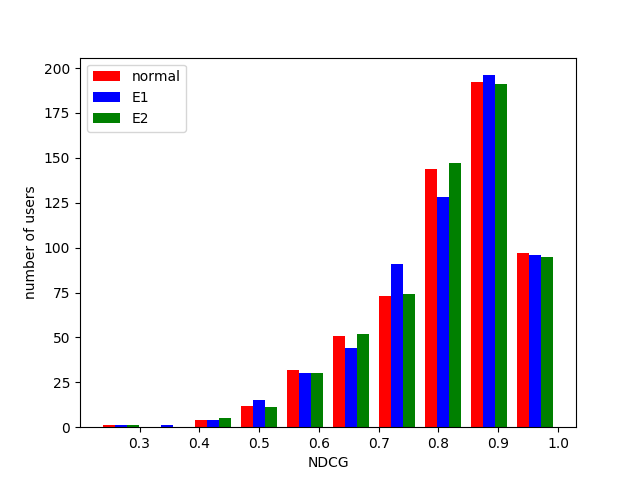
\includegraphics[bb=0 0 360 270, width=\hsize]{img/hist.png}
		\caption{各モデルにおける各ユーザーの精度分布}
	\end{figure}
	
	また, 各モデルにおける推薦因子の寄与分を視覚化することでモデルの特徴を掴む(図2). 
	最後に, 推薦結果がどのくらい異なるのか検証するために3つのモデルのtop20の推薦リストを比べると, normalと比較して
	$E_h^{(1)}$を重視したモデルは平均7.95個, $E_h^{(2)}$を重視したモデルは平均1.01個の新しいアイテムがおすすめされた. そこで参考に, あるユーザーに対してのtop10の推薦リストを以下に記載した(表7). 
	
	\begin{figure}[H]
		\centering
		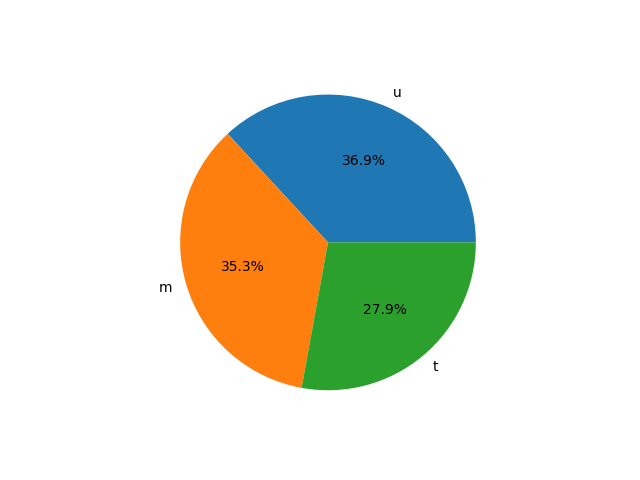
\includegraphics[bb=0 0 360 270, width=\hsize]{img/normal.png}
	\end{figure}
	
	\begin{figure}[H]
		\centering
		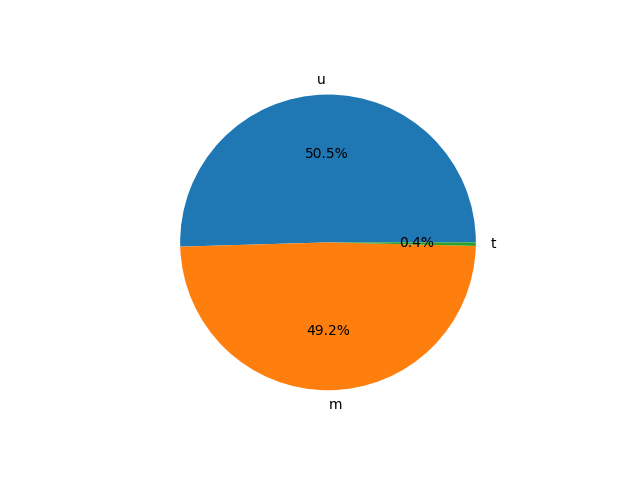
\includegraphics[bb=0 0 360 270, width=\hsize]{img/e1.png}
	\end{figure}
	\begin{figure}[H]
		\centering
		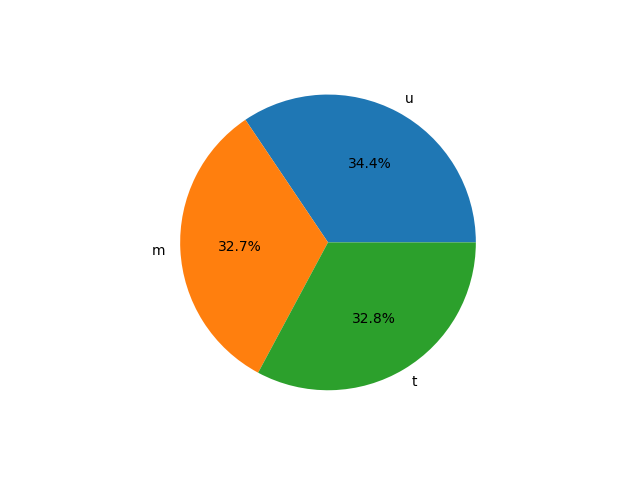
\includegraphics[bb=0 0 360 270, width=\hsize]{img/e2.png}
		\caption{各モデルにおける推薦因子の寄与分. 上段: normal 中段: $E_h^{(2)}$ 下段: $E_h^{(3)}$ }
	\end{figure}
	
	
	
	\begin{table}[htbp]
		\centering
		\caption{Top10の推薦リスト}
		\scalebox{0.4}{
			\begin{tabular}{llll}\hline
				UserID&normal&$E_h^{(1)}$&$E_h^{(2)}$ \\ \hline
				1 & 924:A Space Odyssey &318:Shawshank Redemption&7020:Proof \\
				&293:Léon&589:Terminator&924:A Space Odyssey \\
				&7361:Eternal Sunshine of the Spotless Mind&150:Apollo 13&293:Léon \\
				&4878:Donnie Darko&32:Twelve Monkeys&7361:Eternal Sunshine of the Spotless Mind \\
				&79132:Inception&380:True Lies&4878:Donnie Darko \\
				&72998:Avatar&588:Aladdin&79132:Inception \\
				&135536:Suicide Squad&858:Godfather&72998:Avatar \\
				&1921:Pi&377:Speed&135536:Suicide Squad  \\
				&3676:Eraserhead&165:Die Hard: With a Vengeance&1921:Pi  \\
				&4226:Memento&364:Lion King&3676:Eraserhead  \\ \hline 
				132&924:A Space Odyssey &110:Braveheart &924:A Space Odyssey \\
				&6327:Decade Under the Influence &527:Schindler's List &6327:Decade Under the Influence \\
				&72998:Avatar &150:Apollo 13 &72998:Avatar \\
				&1921:Pi &480:Jurassic Park &1921:Pi \\
				&135536:Suicide Squad &589:Terminator  &3676:Eraserhead \\
				&3676:Eraserhead &457:Fugitive &7932:Dark Days \\
				&4144:In the Mood For Love &590:Dances with Wolves &135536:Suicide Squad  \\
				&541:Blade Runner &1198:Raiders of the Lost Ark &4144:In the Mood For Love \\
				&2762:Sixth Sense &780:Independence Day &541:Blade Runne \\
				&122912:Avengers: Infinity War &608:Fargo  &2762:Sixth Sense\\ \hline
				606&7936:Shame  &150:Apollo 13 &7936:Shame \\
				&135536:Suicide Squad &457:Fugitive &135536:Suicide Squad \\
				&4878:Donnie Darko &608:Fargo &1288:This Is Spinal Tap  \\
				&79132:Inception &380:True Lies &4223:Enemy at the Gates \\
				&1288:This Is Spinal Tap &588:Aladdin  &112552:Whiplash \\
				&112552:Whiplash &377:Speed &4878:Donnie Darko \\
				&4223:Enemy at the Gates &364:Lion King &79132:Inception \\
				&122912:Avengers: Infinity War &595:Beauty and the Beast &122912:Avengers: Infinity War \\
				&99114:Django Unchained &344:Ace Ventura: Pet Detective &6235:Europa Europa \\
				&6235:Europa Europa &165:Die Hard &99114:Django Unchained \\ \hline
			\end{tabular}
		}
		
	\end{table}
	\newpage
	\section{考察}
	表2, 3からエッジの重みを大きくすることでエッジの重要度が上がり, そのエッジに繋がる因子の寄与分が変化し推薦因子を変えることができたことがわかる.また, 第5.4.2章をみると, どのモデルについてもnormalと比較して, 表4よりシステム全体の精度に大きな違いはないが, 表5のMANDをみるとユーザーごとの精度に僅かな違いがあることがわかる. また, 表6でモデルごとの最も高い精度を出したユーザーの数を比較したところ, 結果に大きな偏りがない. 
	つまり, 推薦モデル間でシステムとしての精度に大きな違いはないが, normalが最も精度が高いユーザーもいれば, いずれかのエッジ$E_h^{(t)}$の重みを大きくしたモデルが
	最も精度が高いユーザーもいるということである. このことから, ユーザーごとに適する推薦モデルが異なることがわかる. 
	また, 図2の各モデルにおける推薦因子の寄与分をみると, 各モデルの特徴が異なることがわかる. 
	以上のことから, 推薦因子の寄与分が異なるそれぞれの推薦モデルがユーザーの好みを表現できたと考えられる. 
	また, 表5と図1をみると, normalと比較して$E_h^{(1)}$を重視したモデルでは結果に違いが出るのに対して, $E_h^{(2)}$を重視したモデルでは大きな変化がないことがわかる. 第4.3章や表2, 3からわかるように$E_h^{(2)}$の重みを大きくしたとき, 推薦因子の寄与分があまり変化していないことが原因であると考えられる. 
	表7の推薦結果においても同様で, $E_h^{(1)}$を重視したモデルでは推薦結果が変わるが, $E_h^{(2)}$を重視したモデルではほとんど変わらないことがわかる. 
	表7からは, ユーザーによって推薦結果が異なることもわかる. 
	\\ 最後に, 今回の実験の結果からユーザーによって最適な推薦モデルが異なることがわかり, 
	提案した手法によって, 推薦モデルがユーザーの好みを表現するパーソナライズな推薦の可能性が示されたと言える.  
	\newpage
	\section{おわりに}
	本稿では, ソーシャル情報であるユーザーやアイテム, タグなどの複数のオブジェクトとそれらの関係性を用いて推薦するとき, ユーザーによって重視する関係性が異なると考え, 
	関係性に重みを付けてユーザーの好みを表現するパーソナライズな推薦モデルを提案した. 具体的には, ソーシャル情報をハイパーグラフでモデル化するとき, 
	関係性を表現するエッジの重みを調整することで, 推薦結果における推薦因子の寄与分を変化させ, 推薦モデルがユーザーの好みを表現できるか検証した. 
	実験の結果から, 推薦因子の寄与分が異なる推薦モデル間において, 推薦の精度に大きな違いはないが, ユーザーによって最適な推薦モデルが異なり, 推薦モデルがユーザーの好みを表現するパーソナライズな推薦の可能性が示された. 
	\\ 今後の課題として, 他のデータセットを用いた実験, 各ユーザーそれぞれに適したモデルで推薦することによるシステム全体の精度の向上, 
	それぞれのモデルの推薦結果を組み合わせることによる推薦結果の多様性の向上などの検討が挙げられる. 
	
	\newpage
	\section*{謝辞}
	\addcontentsline{toc}{section}{\numberline{}謝辞}
	本研究を行うにあたり,北海道大学大学院情報科学研究科情報理工学専攻数理科学講座
	情報認識学研究室の中村篤祥准教授には,研究テーマの設定から方針,内容について貴重
	な教示を賜りましたことを,深く御礼申し上げます.また,工藤峰一教授には貴重な御意見を頂きましたことを深く御礼申し上げます.最後に,同研究室の先輩方には
	研究や発表を含め様々な御指導, 御協力に感謝致します. 
	\newpage
	%\section*{参考文献}
	\small
	\addcontentsline{toc}{section}{\numberline{}文献}
	\bibliography{ref}	


\end{document}
